\section{Population theory}\label{sec:population}

\subsection{Model and assumptions}

All quantities below may depend on $n$: the dimension $p=p_n$, the
tail-index function $\gamma$, the active set $\A$, its size $s=|\A|$, and
later the bandwidth $h$, the tail fraction $\alpha$ and the retained size
$d$. The index $n$ is suppressed whenever no ambiguity arises.

\emph{Notation.} A positive measurable function $f$ is slowly varying
at infinity if $f(ty)/f(y)\to1$ as $y\to\infty$ for every $t>0$, and a
survival function $\bar F$ is regularly varying with index $-1/\xi<0$
if $\bar F(ty)/\bar F(y)\to t^{-1/\xi}$ for every $t>0$. Generalized
inverses are $F^{-1}(t)=\inf\{y:F(y)\ge t\}$. For $u\in[0,1]$ and
$v\in[0,1]^{p-1}$, $\iota_j(u,v)\in[0,1]^p$ denotes the vector with
$u$ in coordinate $j$ and $v$ in the remaining coordinates, in order;
we abbreviate $\gamma(u,v)=\gamma\{\iota_j(u,v)\}$ when $j$ is clear
from context. Norms on $[0,1]^{\A}$ are Euclidean. All asymptotic
statements concern a triangular array indexed by $n$, and
$Z_n=O_{\Pp}(a_n)$ means $\lim_{C\to\infty}\limsup_n
\Pp(|Z_n|>Ca_n)=0$.

The observed data are i.i.d.\ pairs $(X_i,Y_i)$ with $Y_i>0$ and
$X_i\in\R^p$ with continuous marginal distribution functions
$F_1,\ldots,F_p$. The theory is formulated on the latent
probability-integral transforms $U_{ij}=F_j(X_{ij})$, so that
$U_i\in[0,1]^p$ has uniform one-dimensional marginals and unrestricted
cross-coordinate dependence; the transforms are never needed by the
algorithm, because the ranks of $X_{1j},\ldots,X_{nj}$ coincide with the
ranks of $U_{1j},\ldots,U_{nj}$ almost surely. With slight abuse of
notation we write $\gamma$ for the tail-index function on the cube,
$\gamma(u)=\gamma_X\{F_1^{-1}(u_1),\ldots,F_p^{-1}(u_p)\}$, where
$\gamma_X$ is the function appearing in \eqref{eq:intro-rv}.

\begin{itemize}
\item[(C1)] \emph{Conditional regular variation.} For every $u$, the
conditional survival function factorizes as
\[
 \bar F(y\mid u)=\Pp(Y>y\mid U=u)=y^{-1/\gamma(u)}L(y,u),
\]
where $L(\cdot,u)$ is slowly varying at infinity,
$\gamma:[0,1]^{p}\to(0,\infty)$ is continuous, and
$0<\underline\gamma\le\gamma(u)\le\Gamma<\infty$ uniformly in $n$ and
$u$.
\item[(C2)] \emph{Uniform tail regularity.} There is a function $c$ with
$0<c_-\le c(u)\le c_+<\infty$ such that
$\sup_u|L(y,u)/c(u)-1|\to0$ as $y\to\infty$.
\end{itemize}
(C1) states that each conditional law is heavy-tailed with index
$\gamma(u)$, as in \eqref{eq:intro-rv}; (C2) strengthens the slow
variation of $L$ to uniform convergence toward a bounded positive limit,
the form needed to control mixtures of the conditional laws.

The active set $\A$ collects the coordinates on which $\gamma$
genuinely depends: $j\in\A$ if and only if there exist $u,v$ differing
only in coordinate $j$ with $\gamma(u)\ne\gamma(v)$. Iterating over the
complementary coordinates shows that $\gamma(u)=g(u_{\A})$ for some
function $g$, and that $\A$ is the smallest coordinate set with this
property. Membership in $\A$ concerns the limiting exponent
only, so a coordinate may shift the body of the conditional distribution, or
its second-order behaviour, without being active. Conditions (C1)--(C2)
parallel conditions (C.1)--(C.2) of \citet{gardesPodgorny2025}, except that
we do not assume the law of $\gamma(U)$ to be absolutely continuous; the
projection argument below handles atoms, which arise as soon as one
coordinate is inactive.

Fix a trimming parameter $0<\varepsilon<1/2$ and write
$\I=[\varepsilon,1-\varepsilon]$. For each coordinate $j$, fix a
pointwise conditional distribution $K_j(u,dv)$ of $U_{-j}$ given
$U_j=u$, and define the conditional law of $Y$ given $U_j=u$ to be
compatible with it through the disintegration identity
\[
 \Pp(Y>y\mid U_j=u)=\int\Pp\{Y>y\mid U=(u,v)\}\,K_j(u,dv);
\]
without such pointwise versions the statements below hold for almost
every $u$. Define
\[
 \xi_j(u)=\esssup\nolimits_{v\sim K_j(u,\cdot)}\gamma(u,v),
\]
the essential supremum of $v\mapsto\gamma(u,v)$ under $K_j(u,\cdot)$;
Proposition~\ref{prop:projection} shows that the conditional law of $Y$
given $U_j=u$ is regularly varying with index $-1/\xi_j(u)$, so
$\xi_j(u)$ is its tail index. One further condition is used only where
stated:

\begin{itemize}
\item[(S)] \emph{Full fibre support.} For every $j$ and $u\in\I$, the
support of $K_j(u,\cdot)$ is all of $[0,1]^{p-1}$. A continuous joint
density, positive on the interior cube, is sufficient.
\end{itemize}

\subsection{Projection turns the surface into an envelope}

Conditioning on $U_j=u$ mixes the conditional laws of $Y$ over the
fibre $\{u\}\times[0,1]^{p-1}$. Heuristically, the slowest-decaying
component of a mixture of heavy tails dictates the tail of the mixture,
so the projected index should equal the largest tail index available on
the fibre, and a localized region of heavy tails should survive
projection intact. The following proposition makes this precise.

For a sub-$\sigma$-field $\mathcal G$, the conditional essential
supremum $\esssup\{\gamma(U)\mid\mathcal G\}$ is the smallest
$\mathcal G$-measurable random variable dominating $\gamma(U)$ almost
surely.

\begin{proposition}[Projection]\label{prop:projection}
Assume (C1)--(C2) and let $\mathcal G\subseteq\sigma(U)$. Then
$\Pp(Y>y\mid\mathcal G)$ is almost surely regularly varying with index
$-1/\xi$, where $\xi=\esssup\{\gamma(U)\mid\mathcal G\}$. In particular
$\xi_j(u)$ is the conditional essential supremum of $\gamma(U)$ given
$U_j=u$. Under (S),
\begin{equation}\label{eq:fibre}
 \xi_j(u)=\max_{v\in[0,1]^{p-1}}\gamma(u,v),\qquad u\in\I.
\end{equation}
\end{proposition}

The essential-supremum identity requires neither full support nor absolute
continuity; (S) enters only to replace the essential supremum by the
maximum over the whole fibre. If dependence removes part of a fibre, the
maximum runs over the conditional support actually available at $u$, and
the population target changes accordingly.

\subsection{Score, gap, and detectability}

Write $\gmax=\max_u\gamma(u)$ for the global maximum and
\begin{equation}\label{eq:score}
 \Psi_j=\frac{1}{1-2\varepsilon}\int_{\I}\xi_j(u)\,du,
 \qquad
 \Delta_j=\gmax-\Psi_j,
 \qquad
 \Delta_{\min}=\min_{j\in\A}\Delta_j.
\end{equation}
The screen ranks coordinates by increasing $\Psi_j$ and keeps the $d$
smallest. Small scores indicate activity: all inactive coordinates share the
flat baseline $\gmax$, while fixing a detectable active coordinate lowers
the attainable envelope. The algorithm uses only the ordering of the
$\Psi_j$ and never estimates $\gmax$.

Let $\M=\argmax_u\gamma(u)$, a nonempty compact set, and let $\pi_j(\M)$ be
its projection onto coordinate $j$.

\begin{proposition}[Detectability]\label{prop:geometry}
Assume (C1)--(C2) and (S).
\begin{enumerate}
\item If $j\notin\A$, then $\xi_j\equiv\gmax$ on $\I$ and $\Delta_j=0$.
\item For every $j$ and $u\in\I$: $\xi_j(u)=\gmax$ if and only if
$u\in\pi_j(\M)$.
\item $\Delta_j>0$ if and only if $\I\setminus\pi_j(\M)$ has positive
Lebesgue measure.
\end{enumerate}
If the restriction of $\gamma$ to the active coordinates has a finite set
of maximizers, every active coordinate is detectable.
\end{proposition}

Claim 3 separates two failure modes that finite-sample experiments tend to
blur. When $\pi_j(\M)$ covers $\I$, no sample size makes coordinate $j$
identifiable from this score; the diagonal example
$\gamma(u_1,u_2)=\gamma_0-(u_1-u_2)^2$, with $\M=\{(t,t):0\le t\le1\}$, is
of this kind, and both of its active coordinates are invisible. When
$\pi_j(\M)$ misses a set of positive measure, detection is a question of
estimation accuracy, quantified by
Section~\ref{sec:estimation}. Figure~\ref{fig:population-profiles}
contrasts the two situations.

\begin{figure}[t]
\centering
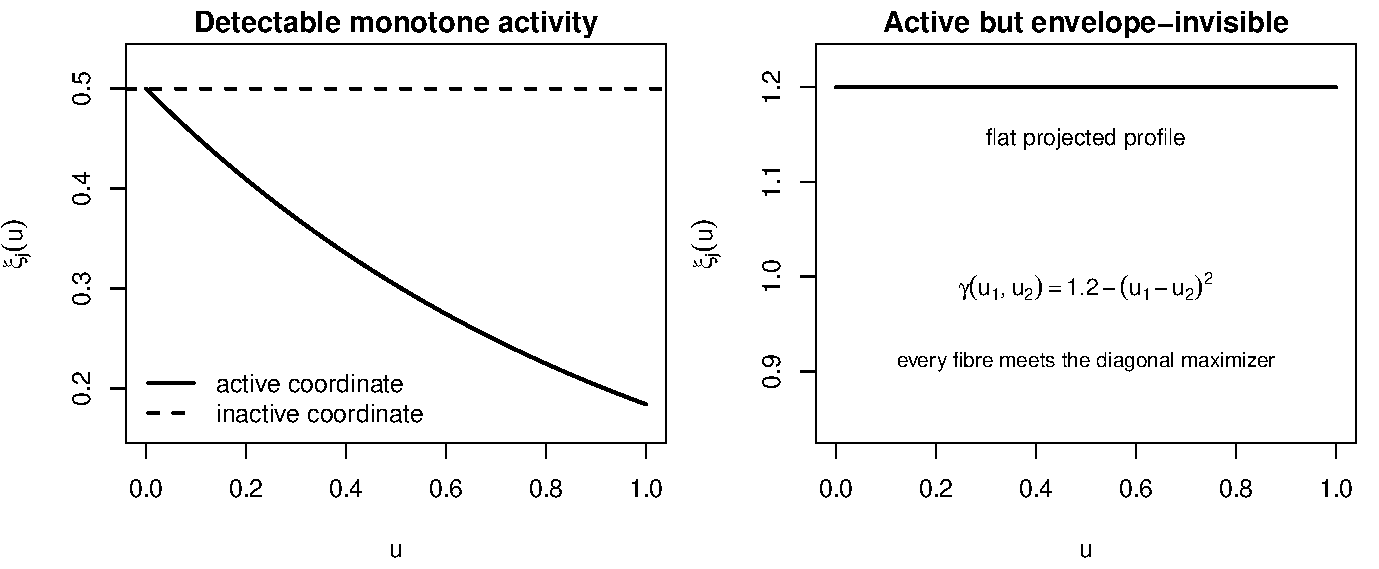
\includegraphics[width=.88\linewidth]{figures/population_profiles.pdf}
\caption{Projected envelopes. Left: a monotone active coordinate depresses
the envelope below the inactive baseline $\gmax$. Right: in the diagonal
example every fibre meets the argmax set, so the envelope of an active
coordinate stays flat.}
\label{fig:population-profiles}
\end{figure}

\begin{proposition}[Quantitative margin]\label{prop:margin}
Assume (C1)--(C2), (S), and that for some $u^\star_{\A}\in[0,1]^{\A}$ and $\nu>0$,
\[
 \gamma(u)\le\gmax-c_1\,\|u_{\A}-u^\star_{\A}\|^\nu
 \qquad\text{for all }u,
\]
for some constant $c_1>0$. Then, for $j\in\A$,
\[
 \gmax-\xi_j(u)\ge c_1\,|u-u_j^\star|^\nu,
 \qquad
 \Delta_j\ge c_1\,\E\bigl(|W-u_j^\star|^\nu\bigr),\quad
 W\sim\mathrm{Unif}(\I).
\]
For $\nu=2$ the right-hand side is at least
$c_1\{(1-2\varepsilon)^2/12+(1/2-u_j^\star)^2\}$.
\end{proposition}

Two consequences of \eqref{eq:fibre} help with examples. If
$\gamma(u)=G(\sum_{\ell\in\A}g_\ell(u_\ell))$ with $G$ strictly increasing,
then $\xi_j(u)=G(g_j(u)+\sum_{\ell\in\A,\,\ell\ne j}\max g_\ell)$, and
$\Delta_j>0$ whenever $g_j$ lies below its maximum on a subset of $\I$ of
positive measure. If $\partial_j\gamma\ge c_j>0$ throughout the cube,
arbitrary interactions are allowed and $\Delta_j\ge c_j/2$.

For the benchmark $\gamma(u)=\tfrac12\exp(-u_1-u_2-u_3-u_4)$ used in
Section~\ref{sec:simulation}, $\xi_j(u)=e^{-u}/2$ for $j\le4$ and
$\xi_j\equiv1/2$ otherwise, so $\Delta_j\approx0.186$ at
$\varepsilon=0.05$. The gap is comfortable, yet estimating $\xi_j(u)$ near
its maximum requires sample points whose remaining three active
coordinates are simultaneously small; the simulations keep population
detectability and finite-sample accessibility clearly separated.
